\documentclass{article}
\usepackage{mathtools}
\usepackage{optidef}

\begin{document}

\section{Introduction}

Local Energy Markets (LEMs) are mechanisms by which users in a power grid can exchange energy. The framework assumes that each participant acts on his/hers own best interest, whatever that might be. Because of that, a participant might decide to \textit{play the market game} as they desire. In this technical report we analyze one of the possible dimensions in which players might reason about LEMs and how that reasoning impacts on the grid. 
More specifically, we seek to understand how the players beliefs about future market prices impact the net load seen from the grid.

\section{Model description}

Let $\mathcal{N} = \{1, 2, \dots, N\}$ be the set of consumers participating in the local energy market and $\mathcal{T} = \{1, 2, \dots, T \}$ be the set of discrete timeslots considered.
At each timelot $t$, each consumer $i$ has a load $z^i_t$ which can be positive if they are consuming energy or negative if they are generating more than what they are producing.

Each user has an electricity contract that specifies the price of elecitricity $p^i_t$ for every timeslot $t$. Users can also sell energy at the price $f^i_t$.

The cost of each consumer $C^i$ can be calculated using Equation \eqref{eq:cost_do_nothing}.

\begin{equation}\label{eq:cost_do_nothing}
	C^i = \sum_{t \in \mathcal{T}} \left[ p^i_t\max\{z^i_t, 0\} - f^i_t\max\{ -z^i_t, 0\} \right]
\end{equation}

If users have a battery, they can shift some of their consumption in order to minimize costs. For a user owning a battery, his/shes new optimal consumption is given by the optimization problem defined in \eqref{eq:opt_prob}.

\begin{mini!}[4]
  {x_1, \dots, x_{T}}{C^i = \sum_{t=1}^{T} p^i_t[s_t + z^i_t]^+ - f^i_t[s_t
  + z^i_t]^-}{}{P)}
  \label{eq:opt_prob}
  \addConstraint{b_{j+1} }{= b_j + x_j }{ \ j=1, \ldots,T}
  \addConstraint{s_j}{=\begin{cases} \frac{x_j}{\eta_c} & \text{if } x_j \geq 0 \\ x_j \eta_d & \text{ if } x_j < 0 \end{cases}}{j=1, \ldots, T}
  \addConstraint{x_j }{\in \mathcal{X}(b_j) }{j=1, \ldots,T}
\end{mini!}

where $b_t$ represents the amount of energy stored in the battery at time $t$, $\eta_c, \eta_d \in (0, 1]$ are the charging and discharging efficiencies, $s_t$ is the energy seen from outside the battery taking into account the efficiency coeficients and $\mathcal{X}(b_t)$ defines the set of possible battery actions given the state of charge $b_t$. $\mathcal{X}$ is defined in equation \eqref{eq:feasible_set}, where $\delta_{\min} < 0, \delta_{\max} > 0$ represent the maximum power the battery can provide, $h$ is the length of the timeslot in hours, and $b_{\min}, b_{\max}$ are the minimum and maximum capacities of the battery in kWh.

Observe that the quantity $s_t + z^i_t$ is the amount of energy that player $i$ consumes at time $t$ seen from the grid.

\begin{equation}
  \label{eq:feasible_set}
  \mathcal{X}(b) = \left[\max\{\delta_{\min}h, b_{\min} - b \}, \min\{
  \delta_{\max}h, b_{\max} - b\} \right]
\end{equation}

\subsection{Time frames}

To simulate, we use a receding horizon framework. For each timeslot $t$, each user forecasts his load until the end of the day, solves the optimization problem \eqref{eq:opt_prob} (starting from timeslot $t$ instead of timeslot 1) and implements the first action. He/she trade buy/sell/use the battery as desired during the timeslot and when the timeslot ends, they \textit{move into the next one} and repeat the process. Basically, they use Model Predictive Control with a receding horizon.

\subsection{Markets}

Following most of the literature in LEMs, we model the market as independent auctions occurring once per timeslot. Before the beginning of timeslot $t$, the market organizer collects bids from all the players. It then clears the market using some mechanism(we used a strategy proof double auction) and notifies the players how much of their bid was accepted and at which price.

A bid consists of a pair $(quantity, price) = b = (b_q, b_p)$ that specifies how much energy is desired and at which price.

A market result for a given player is a pair $r = (r_q, r_p)$ where $|r_q| \leq |b_q|$, the quantity traded is equal or less than the desired quantity and $r_p \geq b_p$ if selling or $r_p \leq b_p$ if buying.

\subsection{Timeframes 2}

The integration between the optimal schedule of the consumers and the market is as follows:

At start of timeslot $t'$, user $i$ will
\begin{enumerate}
\item Obtain a forecast of the load until the end of the horizon considered $\hat{z^i_j}, \ j=t',\dots, T$. Forecast the overall price at which he/she will buy ($\hat{p^i}_j$) and sell ($\hat{f^i}_j$)energy until the end of the horizon $j=t', \dots, T$. Note that although the contracted price is fixed, the price resulting from the market is not.
	\item Solve the optimization problem \eqref{eq:opt_prob} using $\hat{p}$ and $\hat{f}$. Let $s^{i*}_{t'}$ denote the first component of the optimal solution.
	\item Bid in the market $b^i_{t'} = (s^{i*}_{t'} + z^i_t, \hat{p}^i_t)$ (or $\hat{f}^i_t$ if selling).
	\item Re-run the optimization problem \eqref{eq:opt_prob} using the real price $p^i_t, f^i_t$ instead of the forecasted version $\hat{p}^i_t, \hat{f}^i_t$. To guarantee consistency with the market result, the problem has the additional constraint $s^{i*}_{t'} + z^i_t \geq r_q$ if buying or $\leq$ if selling. The solution of this new instance in combination with the market result will be the overall action of the player.
\end{enumerate}

\subsection{Forecasting the market price}

For this experiment we are concerned with the impact of the price forecasting technique in the net load consumption. We do not try to find the best techniques but rather, to see if a simple and \textit{naive} method would be enough to cause problems in the grid.

To do so, we consider 3 different techniques for forecasting the prices: \textbf{Do Nothing}, \textbf{Last Clearing Price}, \textbf{Last Price Paid}. In the first one, users do not forecast the market price and therefore plan their schedule as if the market did not existed. In the second one, the prices only forecast the prices of the next time slot $t' + 1$ using the clearing price of the market in timeslot $t'$, that is: $p^i_{t' + 1} = f^i_{t' + 1} = cp_{t'}$, where cp is the clearing price. Finally, in the last case, $p^i_{t' + 1} = f^i{t' + 1} = pp_{t'}$ where pp stands for the actual price paid for energy. That is, if all the energy was traded in the market, it is the same as the second method; if all the energy was traded with the utility is equivalent to the first, but if some energy was bought in the market and some from the utility is the weighted average of the prices paid.

Observe that the forecast is only one timeslot ahead. For the remaining timeslots, the prices are assumed to be the contracted ones. 


\section{Experiment Setup}

Simulations were ran using data from the Ausgrid project, which I had available already. Consumption is sampled every 30 minutes and therefore $T = 48$ (the horizon is one day).
Fifty users were considered, and for all of them we modeled a battery with $b_{\max} = 3, \delta_{\min} = -\delta_{\max} = 1$ and $\eta_c = \eta_d = 0.95$.

All players faced the same price structure with $f^i_t = 5, \ \forall t$, $p^i_t = 10, \ t \in [1, 24]$ and $p^i_t = 15, t \in [25, 48]$.

Because the dataset had very little generation on its own, for half of the players we \textit{added} extra generation. This was done by random sampling a uniform variable between $[-1, 0]$ for timeslots between 15 and 30.

\section{Results}

Figures \ref{fig:img/lastcp2013524}, \ref{fig:img/lastpaid2013524} and \ref{fig:img/donothing2013524} depict the aggregated load, seen from the grid for the three different sets of strategies on the 24th of May 2013. In all pictures, the green curve represents the base load of all users without markets nor batteries, the orange curve depicts the net load with batteries but without the market and finally the blue curve represents the net load with batteries and the market. 
It can be seen that the \textit{Do Nothing} strategy (Figure \ref{fig:img/donothing2013524}) effectively is no different from the scenario without market. Consequently, we turn our attention to the other two plots. 

\begin{figure}[htpb]
	\centering
	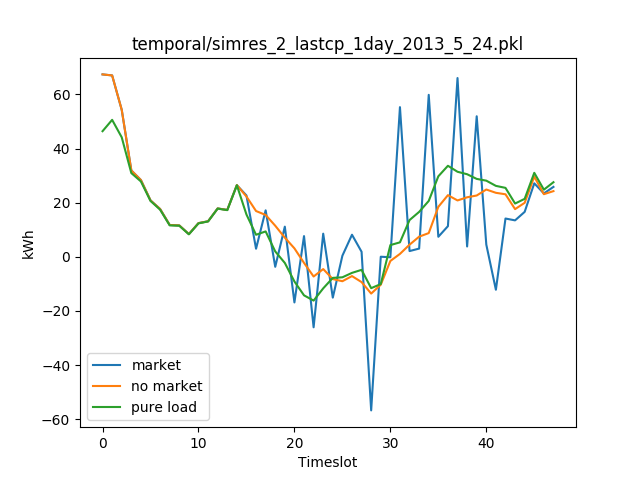
\includegraphics[width=0.8\linewidth]{img/lastcp2013524.png}
	\caption{Aggregated consumption of all players when they use the strategy \textbf{Last Clearing Price}}
	\label{fig:img/lastcp2013524}
\end{figure}


\begin{figure}[htpb]
	\centering
	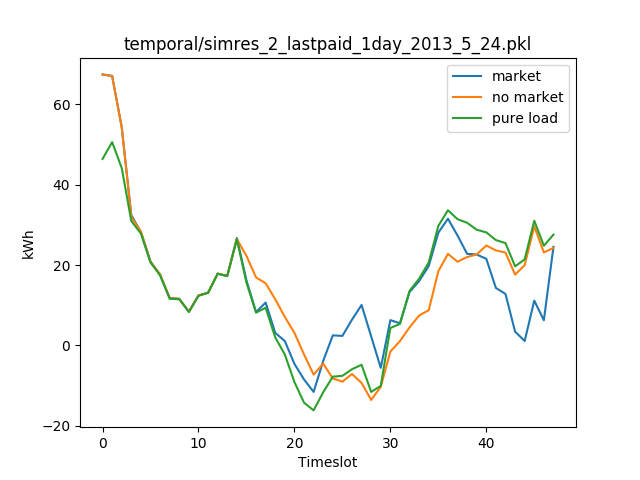
\includegraphics[width=0.8\linewidth]{img/lastpaid2013524.png}
	\caption{Aggregated consumption of all players when they use strategy \textbf{Last Paid Price}}
	\label{fig:img/lastpaid2013524}
\end{figure}

\begin{figure}[htpb]
	\centering
	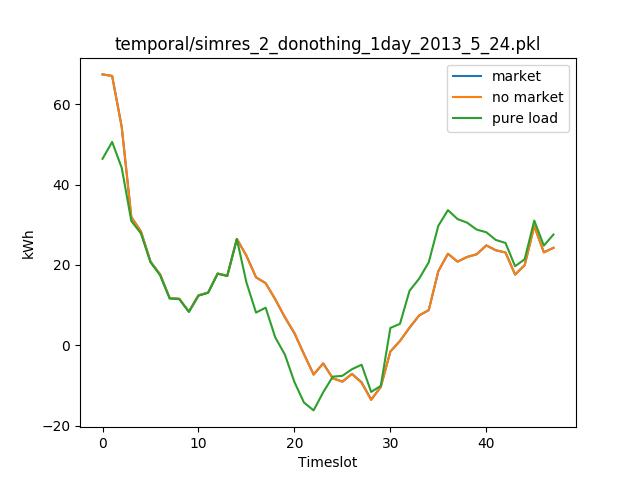
\includegraphics[width=0.8\linewidth]{img/donothing2013524.png}
	\caption{Aggregated consumption of all players when they use strategy \textbf{Do Nothing}}
	\label{fig:img/donothing2013524}
\end{figure}

Strategy \textbf{Last Clearing Price} offers the greater variability, as it can be seen in the huge spikes for both, consumption and injection of power. In what follows, we show insight in why that occurs.

\subsection{Analysis of the Last Clearing Price Strategy}

From time slots 1 to 15, all the bids were buying bids. Consequently, no trade occured. This is consisten with the orange and the green curve in Figure \ref{fig:img/lastcp2013524} being the same at the beginning.







\end{document}
